\chapter{Projektowanie Bazy Danych}
Projekt: baza danych dla sklepu internetowego sprzedającego akcesoria kuchenne\\
Obecnie zamawiający SZBD sprzedaje towar na popularnym serwisie aukcyjnym.\\ 
\section{Sformułowanie celu i zadań}
Cele:
\begin{enumerate}
\item Minimalizacja czasu
\begin{itemize}
\item pomiędzy złożeniem zamówienia przez klienta a przekazaniem towaru do wysyłki w przypadku wysyłki za pobraniem
\item pomiędzy zaksięgowaniem wpłaty klienta a przekazaniem towaru do wysyłki w przypadku płatności z góry 
\end{itemize} 
\item Minimalizacja ilości osób zaangażowanych w zarządzanie sprzedażą
\item Ujednolicenie istniejącej bazy produktów i ich kategorii
\item Uniezależnienie się od wykorzystywanego portalu aukcyjnego
\item Automatyzacja wystawiania faktur / rachunków
\item Zapewnienie łatwej kontroli nad aktualnymi stanami magazynowymi produktów 
\end{enumerate}

\subsection{Analiza istniejacej bazy — analiza stanu wyjsciowego}
Zamawiający SZBD sprzedaje towar na popularnym serwisie aukcyjnym. 
Ze względu na powiększenie oferowanego asortymentu istniejący model funkcjonowania przedsiębiorstwa przestaje być wystarczająco wydajny 
ze względu na źle przemyślany schemat przechowywania danych
\begin{enumerate}
\item opisy produktów jako pliki tekstowe przechowywane w strukturze katalogowej odpowiadającej kategoriom
\item stany magazynowe w arkuszu kalkulacyjnym (bez multidostępu do zapisu)
\item ceny w arkuszu kalkulacyjnym
\item rozliczenia roczne też 
\item dokumenty (np. faktury, raporty z przekazania do wysyłki) w formie papierowej - opisać dokładniej
\item baza kupujących przechowywana jest przez system aukcyjny	
\end{enumerate}
\textbf{W jaki sposób baza jest wykorzystywana?}\\
Aby dodać produkt do sprzedaży, wyszukiwany jest odpowiedni plik tekstowy z jego opisem oraz sprawdzane cena i stan magazynowy w arkuszu kalkulacyjnym.
Kategoria ustalana jest ręcznie w arkuszu kalulacyjnym zawierającym stany magazynowe
Produkty są wystawianie ręcznie na popularnym serwisie aukcyjnym.
Informacje o kupnie: jaki towar, w jakiej ilości, w jakiej cenie oraz o wpłacie dostarczane są przez serwis aukcyjny w formie tekstowej (elektronicznie)
Do osoby odpowiedzalnej za gromadzenie towaru w paczkę do wysyłki i przekazanie paczki kurierowi przekazywana jest w formie wydruku
Informacje potrzebne do generowania raportów przepisywane są do arkusza kalkulacyjnego ręcznie.
Problemy: 
\begin{enumerate}
	\item żmudne wyszukiwanie danych
	\item duże ryzyko ludzkiego błędu podczas ręcznego przenoszenia danych 
\end{enumerate}


\subsection{Lista pól w projektowanej bazie}
\begin{enumerate}
\item klient: klient\_id, typ(firma/os.prywatna) nazwisko, imię, NIP, nazwa\_firmy, domyślny\_adres\_wysyłki, login, hasło
\item kategoria: kategoria\_id, nazwa, id\_nadrzednej
\item produkt: produkt\_id, nazwa, opis, stan\_magazyn, cena, blokada

\item rabaty\_klient: klient\_id, kategoria\_id, wysokosc\_rabatu 
\item promocje\_produkt: produkt\_id, klient\_id, wysokosc\_rabatu , data\_od, data\_do 

\item transakcje: transakcja\_id, klient\_id, adres\_wysyłki, kwota\_zamowienia, kwota\_wplacona, status
\item produkty\_zakupione (bezpośrednio związane z transakcj): transakcja\_id, (wszystkie pola produkt), ilość
koszyk

\item najwazniejsze: konta
\end{enumerate}
\subsection{Związki między elementami:}
\begin{itemize}
\item Kategorie są wielopoziomowe (z podkategoriami)
\item Produkt należy tylko do jednej (pod)kategorii
\item Dane produktów mogą zmieniać się w każdej chwili
\item Dla każdej transakcji należy przetrzymywać informacje o produkcie z momentu wyświetlenia podsumowania zamówienia klientowi
\item Raport podsumowujący transakcję przed "zatwierdzam i płacę" = świętość, dane tam nie mogą ulec zmianie przez modyfikację parametrów produktu (w szczególności: cena)
\item Użytkownik niezalogowany ma możliwość zrobienia zakupów w sklepie internetowym
\end{itemize}

\subsection{Diagram przypadków użycia}

\begin{figure}
	\centering
	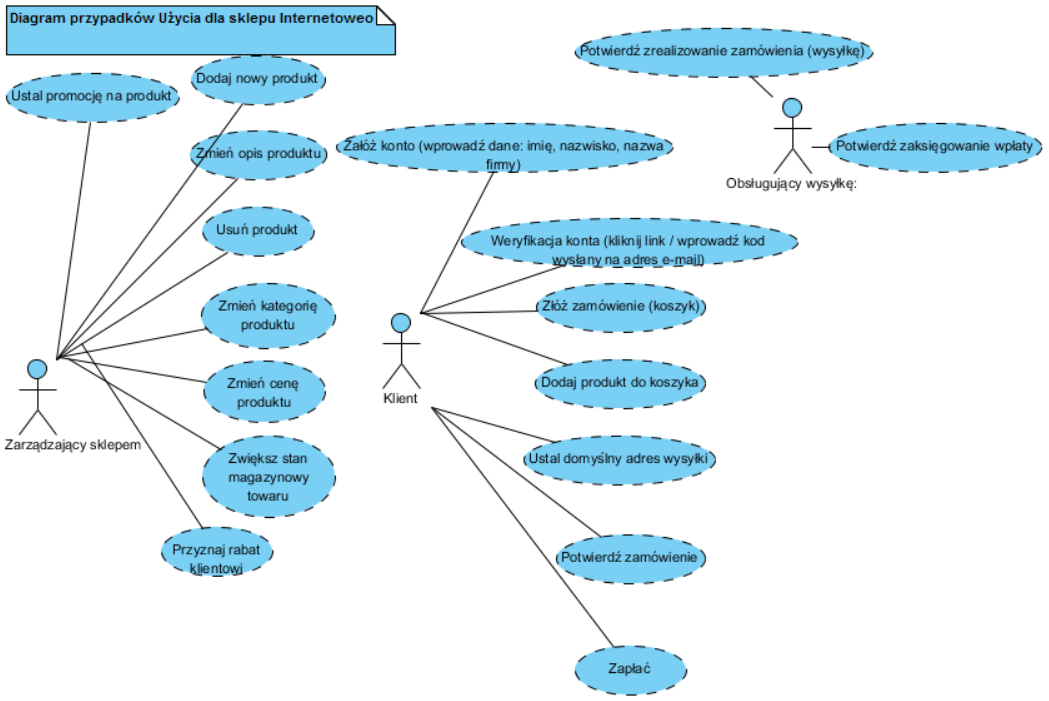
\includegraphics[width=15 cm] {fig/use_case_diagram}
	\caption{Diagram przypadków uycia}
	\label{fig:use_case_diagram}
\end{figure}
\subsection{Diagram klas}
\begin{figure}
	\centering
	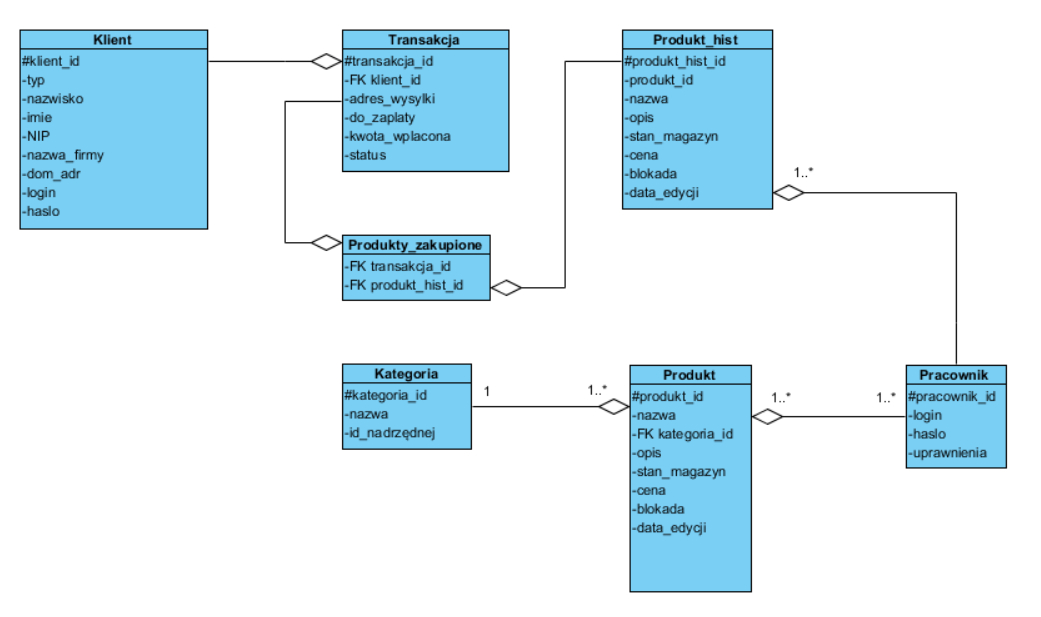
\includegraphics[width=15 cm] {fig/klasy}
	\caption{Diagram klas}
	\label{fig:diagram klas}
\end{figure}
\subsection{Wyjściowa funkcjonalność}
\section{Definiowanie tabel, wiezów integralnosci, perspektyw}